\documentclass[12pt, openany]{book}

% ──────────────────────────────────────────────
% Packages
% ──────────────────────────────────────────────
\usepackage[margin=1in]{geometry}
\usepackage{amsmath, amssymb, amsthm}
\usepackage{mathtools}
\usepackage{bm}
\usepackage{graphicx}
\usepackage{tikz}
\usepackage{pgfplots}
\pgfplotsset{compat=1.18}
\usetikzlibrary{arrows.meta, decorations.markings, calc, patterns, positioning,
  3d, perspective}
\usepackage{tcolorbox}
\tcbuselibrary{theorems, breakable, skins}
\usepackage{hyperref}
\usepackage{enumitem}
\usepackage{fancyhdr}
\usepackage{titlesec}
\usepackage{epigraph}
\usepackage{xcolor}
\usepackage{booktabs}

% ──────────────────────────────────────────────
% Colors
% ──────────────────────────────────────────────
\definecolor{chapblue}{RGB}{0, 70, 130}
\definecolor{accentred}{RGB}{180, 40, 40}
\definecolor{softgray}{RGB}{245, 245, 245}
\definecolor{trajgreen}{RGB}{30, 130, 60}
\definecolor{darkgold}{RGB}{160, 120, 20}
\definecolor{purplehaze}{RGB}{100, 40, 140}

% ──────────────────────────────────────────────
% Theorem environments
% ──────────────────────────────────────────────
\newtcbtheorem[number within=chapter]{principle}{Principle}{
  colback=chapblue!5, colframe=chapblue!80,
  fonttitle=\bfseries, separator sign={.~},
  breakable
}{princ}

\newtcbtheorem[number within=chapter]{keyidea}{Key Idea}{
  colback=accentred!5, colframe=accentred!70,
  fonttitle=\bfseries, separator sign={.~},
  breakable
}{idea}

\newtcbtheorem[number within=chapter]{example}{Example}{
  colback=softgray, colframe=black!40,
  fonttitle=\bfseries, separator sign={.~},
  breakable
}{ex}

\newtcbtheorem[number within=chapter]{definition}{Definition}{
  colback=darkgold!5, colframe=darkgold!80,
  fonttitle=\bfseries, separator sign={.~},
  breakable
}{def}

\newtcbtheorem[number within=chapter]{remark}{Remark}{
  colback=purplehaze!5, colframe=purplehaze!60,
  fonttitle=\bfseries, separator sign={.~},
  breakable
}{rem}

\theoremstyle{plain}
\newtheorem{proposition}{Proposition}[chapter]
\newtheorem{theorem}{Theorem}[chapter]
\newtheorem{lemma}[theorem]{Lemma}
\newtheorem{corollary}[theorem]{Corollary}

% ──────────────────────────────────────────────
% Chapter formatting
% ──────────────────────────────────────────────
\titleformat{\chapter}[display]
  {\normalfont\huge\bfseries\color{chapblue}}
  {\chaptertitlename\ \thechapter}{20pt}{\Huge}
\titlespacing*{\chapter}{0pt}{-20pt}{30pt}

% ──────────────────────────────────────────────
% Header/Footer
% ──────────────────────────────────────────────
\pagestyle{fancy}
\fancyhf{}
\fancyhead[LE,RO]{\thepage}
\fancyhead[RE]{\textit{Control Is Motion}}
\fancyhead[LO]{\textit{\nouppercase{\leftmark}}}
\renewcommand{\headrulewidth}{0.4pt}

% ──────────────────────────────────────────────
% Custom commands
% ──────────────────────────────────────────────
\newcommand{\state}{\bm{x}}
\newcommand{\control}{\bm{u}}
\newcommand{\traj}{\bm{\gamma}}
\newcommand{\manifold}{\mathcal{M}}
\newcommand{\configspace}{\mathcal{Q}}
\newcommand{\statespace}{\mathcal{X}}
\newcommand{\controlspace}{\mathcal{U}}
\newcommand{\tube}{\mathcal{T}}
\newcommand{\Reals}{\mathbb{R}}
\newcommand{\dd}{\mathrm{d}}
\newcommand{\dt}{\,\dd t}
\newcommand{\ds}{\,\dd s}
\newcommand{\norm}[1]{\left\lVert #1 \right\rVert}
\newcommand{\inner}[2]{\left\langle #1,\, #2 \right\rangle}
\newcommand{\tangent}{\bm{e}_1}
\newcommand{\normal}{\bm{e}_2}
\newcommand{\binormal}{\bm{e}_3}
\newcommand{\frenet}{\bm{e}}


% ──────────────────────────────────────────────
\begin{document}

% Set chapter counter to 1 so this is Chapter 2
\setcounter{chapter}{1}

\chapter{Curves in State Space}
\label{ch:curves_in_state_space}

\section{What a Curve Describes}

A golf swing has several useful geometric descriptions. The clubhead traces a
curve in three-dimensional physical space. The joint configurations trace a
curve in configuration space. Positions, velocities, and any additional
internal states trace a curve in state space. These descriptions answer
different questions. A bend in a plot of joint angle against angular velocity
is not a bend of the clubhead in metres, and its curvature is not a force.

The purpose of this chapter is to make geometry useful without asking it to
supply missing dynamics. We develop arc length, curvature, moving frames,
local transverse coordinates, and timing constraints. We then connect these
tools to physical acceleration, admissible control, and the impact task.
Geometry specifies a motion's shape within a stated space and metric.
Dynamics determines which timed motions and corrections are possible.
Measurements determine whether a proposed model describes an actual swing.

Throughout the Euclidean calculations, the ambient space is $\mathbb R^d$
with a specified inner product. A prime denotes differentiation with respect
to the displayed curve parameter; a dot denotes physical time. A regular
curve has a nonzero first derivative on the interval under discussion.
Configurations are denoted by $q$, full states by $x$, and a physical point
such as the clubhead by $p$. We use $s$ for arc length and $\lambda$ for a
parameter that need not measure distance.

\subsection{Geometry Depends on the Space and Metric}

Euclidean curvature is invariant under regular reparameterization and rigid
changes of Cartesian frame. It is an extrinsic property of the embedded
curve: it measures how the curve bends in its ambient space. Calling this
``intrinsic'' merely because it does not depend on timing confuses two uses
of geometry. A straight segment and a circular arc of the same length have
the same one-dimensional arc-length metric, although their ambient
curvatures differ.

Changing units without transforming the metric changes the calculation.
For a state $x=(q,\dot q)$, a raw sum of squared positions and velocities has
no universal physical meaning. One possible declared convention is
$z=Sx$, where $S$ contains inverse reference scales, followed by Euclidean
geometry in the dimensionless coordinates $z$. Different scales generally
give different curvature signatures. This is a modeling choice to report
and test, not a coordinate-free marker of skill.

For a positive-definite metric $W$, the squared displacement is
$dx^T W dx$. Under $z=Sx$, the same metric has matrix
$\widetilde W=S^{-T}WS^{-1}$. A constant metric can be handled through a
linear change to orthonormal coordinates. With a position-dependent metric,
ordinary second derivatives are not sufficient: curvature uses the
appropriate covariant derivative. The kinetic-energy matrix $M(q)$ defines
a metric on configuration velocities; it is not automatically a metric on
an augmented state containing velocities, activation, and contact variables.

\section{Regular Parameters and Arc Length}

Let $\gamma:I\rightarrow\mathbb R^d$ be a $C^2$ curve, and let
$h(\lambda)=\|\gamma'(\lambda)\|>0$. Its arc-length function and unit tangent are
\begin{equation}\label{eq:arc_length}
 s(\lambda)=\int_{\lambda_0}^{\lambda}h(\mu)\,d\mu,
 \qquad T(\lambda)=\frac{\gamma'(\lambda)}{h(\lambda)}.
\end{equation}
Because $ds/d\lambda=h>0$, the inverse function theorem gives a local regular
arc-length parameter. In that parameter $\|\gamma'(s)\|=1$ and
$T=\gamma'(s)$. Replacing $\lambda$ by a smooth increasing diffeomorphism
changes the rate of traversal while preserving the oriented curve.
A merely increasing function can have zero derivative and need not preserve
regularity at every point.

For example, $(\cos t,\sin t)$ and $(\cos t^2,\sin t^2)$ trace the same circle
on suitable intervals. The second time parameterization has zero velocity
at $t=0$. Arc-length formulas that divide by speed apply for $t>0$; the
circle's geometry can separately be extended through the starting point.
A temporal stop is not by itself a geometric cusp or an infinite curvature.

A reversal is even more informative. In normalized coordinates, the physical path
$p(t)=(t^2,0)$ has zero curvature on either side of $t=0$, while velocity
vanishes and reverses there. The unit tangent defined by time is undefined
at the reversal. The full mechanical state
$x(t)=(t^2,2t)$ has derivative $(2t,2)$ and is regular at the same instant.
Thus the physical point can stop while the state continues moving. There is
no universal conclusion that the top of a backswing is the point of maximum
curvature in any of these spaces.

If a regular configuration path is parameterized by $\lambda$ and traversed
with $\dot\lambda>0$, its chosen-metric speed is
$\dot s=\|q'(\lambda)\|\dot\lambda$. In particular, $\dot\lambda$ is not
Cartesian speed unless the path is parameterized by physical arc length.
This distinction matters when converting a speed limit into a timing law.

\section{Curvature and Physical Acceleration}

For a unit-speed $C^2$ Euclidean curve,
\begin{equation}\label{eq:curvature_def}
 k(s)=\frac{dT}{ds},\qquad \kappa(s)=\|k(s)\|.
\end{equation}
Differentiating $T^TT=1$ gives $T^Tk=0$. Where $\kappa>0$, the principal
normal is $N=k/\kappa$. At a point with zero curvature, $k$ remains defined
but this particular normal does not. Curvature vanishing on an entire
connected regular interval makes $T$ constant and the curve a straight
segment. Vanishing at one point does not: $(t,t^3)$ has zero curvature at
$t=0$ and bends arbitrarily nearby.

For any regular parameter, differentiating the normalized tangent gives
\begin{equation}\label{eq:curvature_general_n}
 \kappa=\frac{\|(I-TT^T)\gamma''\|}{\|\gamma'\|^2}
 =\frac{\sqrt{\|\gamma'\|^2\|\gamma''\|^2-(\gamma'^T\gamma'')^2}}
 {\|\gamma'\|^3}.
\end{equation}
In three dimensions the numerator of the final expression is
$\|\gamma'\times\gamma''\|$. In two dimensions it is the absolute determinant
of the two derivative vectors. There is no need to invent an ordinary cross
product in arbitrary dimension. The projected-acceleration form also avoids
subtracting two large nearly equal squared quantities, although numerical
error can still dominate near zero speed.

\subsection{A Checkable Ellipse}

For $\gamma(\lambda)=(a\cos\lambda,b\sin\lambda)$ with $a>b>0$,
\begin{equation}
 \kappa(\lambda)=\frac{ab}
 {(a^2\sin^2\lambda+b^2\cos^2\lambda)^{3/2}}.
\end{equation}
The major-axis endpoints $(\pm a,0)$, at $\lambda=0,\pi$, have the largest
curvature $a/b^2$. The minor-axis endpoints $(0,\pm b)$ have the smallest
curvature $b/a^2$. With $a=2$ m and $b=1$ m these are $2$ and $0.25$ inverse
metres. Uniformly changing the rate of traversal preserves these values.
Stretching a circle into this ellipse does not preserve curvature.

\subsection{Where the Speed-Squared Law Applies}

Let $p(s)$ now be a physical position in an inertial Cartesian frame, with
$s$ measured in metres, and let $v=\dot s>0$. The chain rule gives
\begin{equation}\label{eq:centripetal}
 \dot p=vT,\qquad \ddot p=\dot vT+v^2k
 =\dot vT+v^2\kappa N\quad(\kappa>0).
\end{equation}
Here $v^2\kappa$ is a physical normal acceleration in m/s$^2$. The identity
is kinematic: it describes the acceleration of the prescribed motion before
assigning which forces produce it.

For a point mass, Newton's law says
\begin{equation}\label{eq:control_demand}
 m\ddot p=F_{\mathrm{act}}+F_{\mathrm{pass}}+F_{\mathrm{external}}
 +F_{\mathrm{reaction}}.
\end{equation}
Only in a model where the actuator supplies the entire resultant force does
$F_{\mathrm{act}}=m(\dot vT+v^2k)$. Gravity, springs, contact, and constraint
reactions can contribute. A $0.2$ kg mass moving at $20$ m/s on a horizontal
circle of radius $1$ m requires $80$ N inward. In an ideal frictionless
circular guide with no tangential resistance, the guide supplies that force
and does zero work because its force is perpendicular to velocity. No
continuous actuator work is needed to maintain the speed in this model.
That calculation does not show that a golfer supplies zero joint moments.
It shows why resultant acceleration and active effort are different
quantities.

A clubhead is a point on a moving, rotating, possibly flexible body rather
than an isolated point mass with all force applied at that point. For a
rigid model with $p=p(q)$,
\begin{equation}
 \dot p=J_p(q)\dot q,\qquad
 \ddot p=J_p(q)\ddot q+\dot J_p(q,\dot q)\dot q.
\end{equation}
The Jacobian-rate term supplies normal acceleration even at constant joint
speed. Segment force and moment balances, distributed mass, hand wrenches,
and any modeled shaft deflection are needed to interpret measured clubhead
acceleration. Multiplying it by total club mass does not generally recover
the hand force.

For a first-order state equation $\dot x=f(x,u,t)$, the analogous curve
identity concerns $\ddot x$, which may include mechanical jerk and internal
state derivatives. When $u$ is differentiable,
\begin{equation}
 \ddot x=f_xf+f_u\dot u+f_t.
\end{equation}
This is not a generic decomposition of $u$ into tangential and normal
forces. The reference condition remains
$f(\gamma(s(t)),u_*(t),t)=\gamma'(s(t))\dot s(t)$, together with input
admissibility. In an autonomous model the final argument is absent.

\section{Moving Frames and Their Limits}

\subsection{An Oriented Three-Dimensional Frame}

For a $C^3$ regular curve in oriented Euclidean three-space with $\kappa>0$,
define $T=dp/ds$, $N=T'/\kappa$, and $B=T\times N$. Then
\begin{equation}\label{eq:frenet_serret}
 \frac{dT}{ds}=\kappa N,\qquad
 \frac{dN}{ds}=-\kappa T+\tau B,\qquad
 \frac{dB}{ds}=-\tau N.
\end{equation}
The signed torsion is
\begin{equation}
 \tau=\frac{\det[p',p'',p''']}{\|p'\times p''\|^2},
\end{equation}
where the primes in this formula may use any regular parameter. Torsion
requires nonzero curvature. A planar regular curve has zero torsion where
the formula is defined; at an inflection the Frenet normal and torsion may
be undefined even when the original curve is smooth.

For the helix $p(\lambda)=(a\cos\lambda,a\sin\lambda,b\lambda)$ with $a>0$,
\begin{equation}
 \kappa=\frac{a}{a^2+b^2},\qquad \tau=\frac{b}{a^2+b^2}.
\end{equation}
Changing the sign of $b$ reflects the helix and changes the sign of torsion.
Proper rotations and translations preserve both. Blindly applying
Gram--Schmidt to all three derivatives chooses the final vector from the
third derivative's residual; it can produce $-B$ when torsion is negative.
That convention cannot simultaneously be identified with the oriented
binormal $T\times N$ without tracking the sign.

In this physical three-dimensional setting, torsion measures rotation of the
osculating plane per unit distance. Torsion of a normalized state-space curve
has a different ambient space and interpretation. It is not a direct measure
of anatomical rotation or of how a golfer should change the swing plane.

\subsection{Higher Dimensions and Regular Normal Frames}

With sufficient smoothness and independent successive derivatives,
Gram--Schmidt constructs an orthonormal basis for the successive osculating
spaces of a curve in $\mathbb R^d$. A full oriented Frenet frame can be chosen
by orthogonalizing the first $d-1$ independent derivatives and completing the
last vector with a fixed ambient orientation. Its equations have the form
\begin{equation}
 e_i'=-\kappa_{i-1}e_{i-1}+\kappa_i e_{i+1},
 \qquad \kappa_0=\kappa_d=0.
\end{equation}
The first $d-2$ curvatures are positive under the required independence
conditions; the final oriented curvature can have either sign or vanish.
Alternatively, a frame made from all $d$ independent derivatives adopts a
different sign convention. State the convention before comparing signatures.
If only a partial frame is constructed, its last derivative need not remain
inside that partial span. A closed lower-dimensional Frenet system needs an
appropriate containing affine subspace and its own regularity assumptions.

There is a simpler option for local control: choose any smooth orthonormal
normal frame $E(s)$, with $d-1$ columns, satisfying
$T^TE=0$ and $E^TE=I$. Define
\begin{equation}
 c=E^TT',\qquad \Omega=E^TE',\qquad
 T'=Ec,\qquad E'=-Tc^T+E\Omega.
\end{equation}
Differentiating $E^TE=I$ shows that $\Omega$ is skew-symmetric. A parallel
normal frame, often called a Bishop frame, chooses $\Omega=0$ locally along
an interval. It continues through zero-curvature points of a regular curve
where the principal Frenet normal fails. Such a frame still requires an
initial normal orientation; a periodic curve can have a nontrivial change
of normal orientation after one circuit.

The number of normal coordinates is $d-1$, not the actuator count. The
one-input spring example in the previous chapter has four independent
unforced trajectory derivatives at its specified initial state. A single
trajectory is one-dimensional, its osculating span can be larger, and the
union of reachable trajectories is another object again.

\section{Shape Reconstruction and Its Limits}

For continuously differentiable $\kappa(s)>0$ and continuous signed
$\tau(s)$ on an interval,
the three-dimensional Frenet equations, together with $p'=T$, reconstruct a
unit-speed curve once its initial point and oriented frame are specified.
Existence and uniqueness follow from the frame's linear differential
equation and integration of $T$. Without the initial point and frame, the
curve is determined up to a proper rigid motion. Analogous statements in
higher dimensions require a complete consistent curvature list and frame
convention; an arbitrary truncated signature is insufficient.

Congruence is not equality relative to the golf ball. Translating or rotating
a clubhead path can make it miss the ball while preserving its curvature and
torsion. A rigid rotation of normalized position-velocity coordinates need
not even correspond to a physically allowed state transformation. Gravity,
contact, anatomy, and the target frame further restrict useful symmetries.
Neither shape reconstruction nor a similar curvature signature establishes
equal timing, forces, face orientation, or performance.

Where $\kappa>0$, the osculating circle has center $p+N/\kappa$ and radius
$1/\kappa$. It matches local position, tangent, and curvature; the tangent
line and osculating plane supply lower-order geometric descriptions. An
osculating sphere in three dimensions needs additional conditions. Writing
$\rho=1/\kappa$, when $\tau\ne0$ its center is
$p+\rho N+(\rho'/\tau)B$. This follows by requiring successive derivatives
of squared distance to a fixed center to vanish through third order. At
zero torsion the construction may fail or be nonunique, depending on
$\rho'$. It is not an unconditional approximation for every high-dimensional
state curve.

\section{Feasible Timing and Available Forces}

For a chosen configuration path $q=q(\lambda)$,
\begin{equation}
 \dot q=q'\dot\lambda,\qquad
 \ddot q=q''\dot\lambda^2+q'\ddot\lambda.
\end{equation}
Substitution into mechanical dynamics gives the required generalized load:
\begin{equation}\label{eq:curve_path_dynamics}
 M(q)(q'\ddot\lambda+q''\dot\lambda^2)+h(q,q'\dot\lambda)
 =B(q)u+Q_{\mathrm{pass}}+Q_{\mathrm{external}}+J_c^T\eta.
\end{equation}
Here $h$ contains the declared velocity and potential terms, and passive
terms must not be counted twice. The path must satisfy configuration
constraints; its derivatives must satisfy their velocity and acceleration
conditions. Contact reactions $\eta$, friction, actuator bounds, activation
dynamics, and any force-rate limits constrain feasible timing. For an
underactuated system, not every desired generalized load lies in the input
image even if every motor is individually below its limit.

For a fully actuated model, each torque bound can become an inequality in
$\lambda$, $\dot\lambda$, and $\ddot\lambda$. This is the basis of
path-constrained time scaling. It is more informative than assigning a
single curvature cost because it retains gravity, inertia, coupling, and
the available input directions. The configuration path and timing can be
optimized in stages, but their feasibility constraints remain coupled.
Retiming also changes the corresponding full state curve, as shown in the
previous chapter.

A simple point-mass model gives a useful limited speed bound. Suppose the
actuator supplies the entire force, with $\|F\|\le F_{\max}$, and there are
no other forces. On a physical arc-length path,
\begin{equation}
 \dot v^2+(\kappa v^2)^2\le(F_{\max}/m)^2.
\end{equation}
Thus $v\le\sqrt{F_{\max}/(m\kappa)}$ is necessary when $\kappa>0$, but leaves
no force for tangential acceleration at equality. For $m=2$ kg,
$F_{\max}=10$ N, $\kappa=0.5$ m$^{-1}$, and $v=3$ m/s, the normal
acceleration is $4.5$ m/s$^2$ and the remaining tangential bound is
$\sqrt{25-4.5^2}=\sqrt{4.75}$ m/s$^2$. If a guide supplies normal reaction,
the actuator's feasible set is different.

At zero curvature this particular normal-acceleration bound supplies no
speed ceiling. Tangential acceleration, initial and terminal conditions,
velocity limits, power, and the next bend can still limit speed. A
minimum-time exercise based only on normal acceleration can therefore lack
an attained smooth solution or a physically meaningful optimum. Prescribe
the full bounds and endpoint conditions before claiming an optimal law.

\section{Local Phase and Transverse Dynamics}

\subsection{Coordinates in a Tubular Neighborhood}

Let $\gamma(s)$ be a regular embedded unit-speed state curve in a chosen
Euclidean metric, and choose the smooth normal frame $E(s)$ above. In a
sufficiently small neighborhood of an interior segment, write
\begin{equation}\label{eq:frenet_coords}
 x=\gamma(s)+E(s)\xi.
\end{equation}
Nearest-point phase satisfies $T^T(x-\gamma)=0$ there. Local uniqueness
requires more than this stationary equation: the curve must not intersect
itself in the neighborhood, and the coordinate Jacobian must be invertible.
The scalar factor $1-c^T\xi$ in that Jacobian must be nonzero. A smaller
neighborhood may be needed to exclude other closest points. For a circle,
the center has many nearest points and the inward normal coordinates become
singular there. Endpoints require one-sided treatment. A regular local
normal frame does not turn all nearby states into a single global chart.

Let the smooth autonomous dynamics be $\dot x=f(x,u)$ and suppose a feasible
nominal input satisfies
$f(\gamma(s),u_*(s))=v_*(s)T(s)$ with $v_*>0$. Differentiate the coordinate
map and project onto $T$ and $E$:
\begin{equation}\label{eq:curve_exact_transverse}
 \dot s=\frac{T^Tf(x,u)}{1-c^T\xi},\qquad
 \dot\xi=E^Tf(x,u)-\Omega\xi\dot s.
\end{equation}
These equations retain both the phase denominator and the normal-frame
transport. They are coordinate-rate equations; the word ``force'' should
not be assigned to every transport term in a first-order state model.

With $u=u_*(s)+\delta u$, the transverse linearization at $\xi=0$ is
\begin{equation}\label{eq:transverse_lin}
 \dot\xi=A_\perp(s)\xi+B_\perp(s)\delta u
 +O(\|(\xi,\delta u)\|^2),
\end{equation}
where
\begin{equation}
 A_\perp=E^Tf_x(\gamma,u_*)E-v_*\Omega,
 \qquad B_\perp=E^Tf_u(\gamma,u_*).
\end{equation}
All partial derivatives here hold $s$ fixed; nominal phase evolves by
$\dot s=v_*(s)$. For explicitly time-dependent dynamics, include the time
state or derive the corresponding time-dependent coordinate map. A
feedback depending on an independently prescribed clock is also a different
problem from the phase-indexed law assumed here.

There is no universal correction of the form speed squared times a curvature
matrix subtracted from the original Jacobian. Curvature enters the phase
map and chosen frame; transverse stability depends on the actual vector
field, its derivatives, input directions, feedback, and regularity.
Changing the normal basis changes the coordinate matrices consistently,
without changing physical attraction of the orbit.

\subsection{The Same Circle With Opposite Stability}

In a neighborhood of $r=R>0$, consider the planar systems
\begin{equation}
 \dot r=a(r-R),\qquad \dot\theta=\omega>0.
\end{equation}
Every value of $a$ has exactly the same nominal circle, curvature $1/R$,
speed $R\omega$, and nominal time parameterization. Yet radial error evolves
as $e(t)=e(0)e^{at}$: $a<0$ attracts, $a>0$ repels, and $a=0$ is neutral.
Curvature and nominal speed cannot distinguish these cases. The figure uses
$R=2$ and $\omega=1.3$, with initial radii $1.8$ and $2.2$, over four model
time units. Its radial growth rates are $a=-0.3$ and $a=0.3$.

\begin{figure}[htbp]
\centering
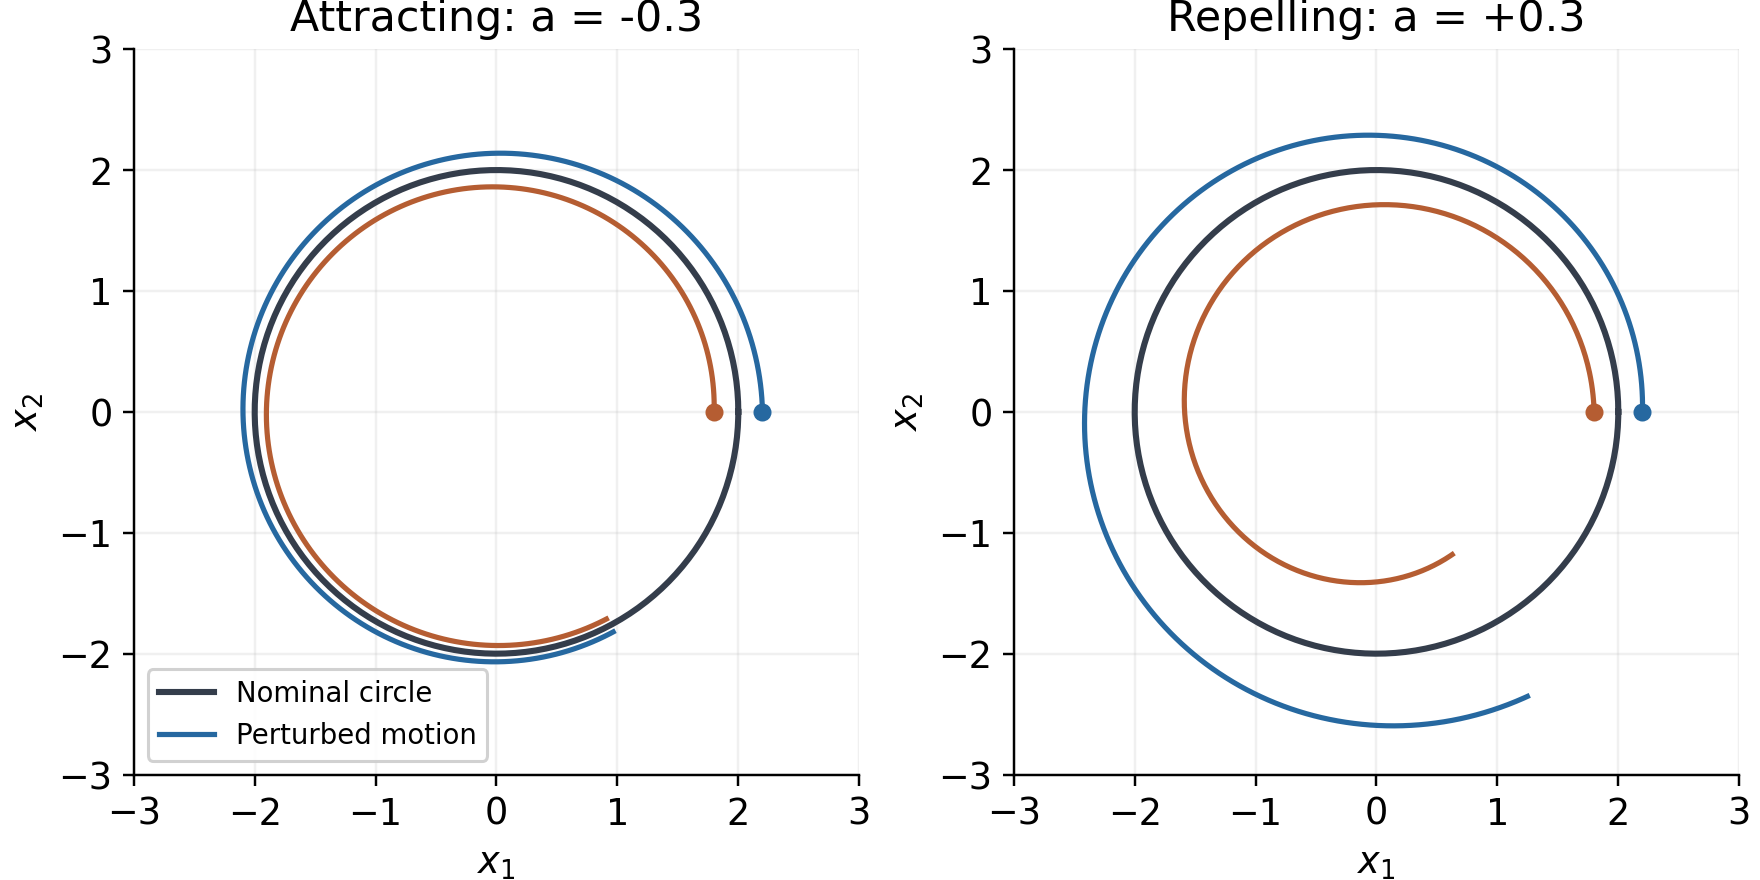
\includegraphics[width=\textwidth]{../The_Geometry_of_Motion/figures/curve_stability_comparison.png}
\caption{The Same Nominal Circle With Opposite Transverse Stability}
\label{fig:curve_stability_comparison}
\end{figure}

Using the inward normal coordinate $\xi=R-r$ and arc length $s=R\theta$
gives $\dot\xi=a\xi$ and $\dot s=R\omega$. The exact phase formula agrees:
$T^Tf=\omega(R-\xi)$ and $1-c^T\xi=1-\xi/R$. Their ratio is $R\omega$.
This checks the denominator as well as the transverse linearization. A
geometric tube around the circle becomes a verified invariant tube only
when the actual transverse dynamics and disturbances satisfy its boundary
condition.

\section{Curvature and Reachability Are Different}

For a control-affine system, instantaneous input directions, reachable sets,
and the derivatives of one trajectory are distinct. Lie brackets describe
noncommuting flows. With the convention
$[g_i,g_j]=Dg_j\,g_i-Dg_i\,g_j$, the bracket can expose a displacement
direction generated by suitable short sequences of controls. The
Chow--Rashevskii result concerns bracket-generating driftless systems under
appropriate smoothness and reversible control assumptions. The orbit
theorem describes the geometry of orbits of vector fields and is not the
same theorem. Allowing forward and backward field flows to define an orbit
does not automatically describe forward-time reachability with drift,
unilateral contact, or bounded controls.

A curved path need not use nonzero brackets at all. For the planar integrator
$\dot x=u$, the two constant input fields commute. The control
$u(t)=(-\sin t,\cos t)$ traces the unit circle from $(1,0)$ with curvature
one. Its acceleration comes from changing the input, while every bracket of
the constant input fields is zero. Conversely, a system can have useful
bracket directions without expressing them as a large curvature along one
recorded trajectory. High curvature does not identify a commutator, a neural
synergy, or an underactuated strategy.

\section{Using Geometry in a Golf Investigation}

A useful investigation keeps the chain of interpretation explicit:
measurement, geometric description, feasible mechanics, uncertainty, and
task outcome. Consider the following protocol.

\begin{enumerate}
\item Choose the object and frame. A clubhead point, shaft orientation,
   joint configuration, and complete state are different data products.
   Use a target-fixed physical frame for ball delivery. State how angles,
   rotations, velocities, and internal states are represented.
\item Report units and metric scales. For a state signature, repeat the
   calculation under plausible scaling choices. For three-dimensional
   clubhead curvature, use physical positions in consistent length units.
\item Fit derivatives with an explicit measurement model. Differentiation
   amplifies noise; torsion requires a third derivative and is especially
   fragile near small curvature or speed. Report sampling, smoothing,
   uncertainty, and sensitivity to filtering. Do not divide by near-zero
   denominators and then interpret numerical spikes as swing phases.
\item Align trials using a declared event or phase convention. Compare both
   geometric shape and timing; report where a reference curve's nearest
   projection becomes ambiguous. Treat impact and contact changes using
   one-sided smooth segments or a hybrid model.
\item Compute physical acceleration and mechanical load with the appropriate
   Jacobians, inertias, external loads, and constraints. Distinguish net
   joint moments from muscle recruitment and resultant force from work.
   Validate these quantities against independent measurements where possible.
\item Evaluate pre-impact speed, face orientation, path direction, strike
   location, and relevant ball outcomes with uncertainty. Test whether a
   geometric feature predicts outcomes beyond simpler measured variables
   on held-out trials. A correlation does not identify the control policy.
\item Test interventions in a declared forward model and then seek empirical
   validation. Altering timing can change speed-dependent loads and contact
   feasibility; altering a path can change moment arms and the impact frame.
   Recompute the complete trajectory rather than attaching a new conclusion
   to an unchanged force history.
\end{enumerate}

The hypothesis that golfers exploit passive coupling remains worth testing.
The geometric tools can identify repeatable patterns and organize model
comparisons. They cannot by themselves establish that a particular pause,
release, curvature peak, or low-dimensional signature is optimal, automatic,
or a consequence of a particular neural strategy. Those arguments require
mechanics and evidence at the next links in the chain.

\section{Further Reading}

The geometric conventions can be checked against
\href{https://www.math.ucla.edu/~petersen/DGnotes.pdf}{Petersen's Classical
Differential Geometry}, especially its curve, Frenet, and parallel-frame
treatments. Path-constrained timing and torque bounds are developed in
\href{https://modernrobotics.northwestern.edu/nu-gm-book-resource/9-4-time-optimal-time-scaling-part-1-of-3/}{Lynch and Park's Modern Robotics}.
For transverse dynamics and orbital stabilization, see
\href{https://arxiv.org/abs/1010.2241}{Manchester's Transverse Dynamics and
Regions of Stability for Nonlinear Hybrid Limit Cycles}. These are
mathematical and robotics references; they do not validate the golf-specific
hypotheses in this chapter.

\section{Exercises}

\begin{enumerate}[itemsep=2pt,parsep=0pt]
\item For $(t,t^3)$, derive the curvature and show why its zero value at the
   origin does not imply a straight neighborhood. Contrast this with the
   stopped physical path $(t^2,0)$ and its regular position-velocity state.
\item Derive the ellipse formula and identify its major- and minor-axis
   endpoint curvatures. Verify invariance under $t\mapsto 2t$ and explain
   why stretching only one coordinate changes the Euclidean answer.
\item Compute curvature and signed torsion for $(t,t^2,t^3)$ at $t=0$ and
   $t=1$. Explain what extra mechanical assumptions are needed to compare
   actuator effort along the two portions of the curve.
\item For the helix $(2\cos t,2\sin t,t)$, calculate $T,N,B,\kappa,\tau$.
   Reflect its third coordinate and track the sign of the oriented torsion.
\item Derive the exact normal-coordinate equations by projecting the
   derivative of $x=\gamma(s)+E(s)\xi$. Identify the coordinate singularity
   for a circle and verify the radial stability counterexample.
\item A $2$ kg point mass is driven solely by a force of norm at most
   $10$ N. Find the available tangential acceleration at speed $3$ m/s on a
   radius-$2$ m circle. Repeat the interpretation when an ideal guide
   supplies all normal reaction.
\item Let $p(\lambda)=\ell(\lambda,\sin(\pi\lambda),0)$ for
   $0\le\lambda\le2$, where $\ell=1$ m. Derive the curvature and the
   conversion from $\dot\lambda$ to physical speed. Formulate a timing
   optimization with a total-acceleration bound, a finite speed bound, and
   zero initial and terminal speeds; do not assume that a bound on normal
   acceleration alone specifies a smooth minimum-time solution.
\item Starting with a declared double-pendulum model, generate a smooth
   swing-like segment and compare configuration, physical clubhead, and
   normalized state curvature. Repeat under different state scales and
   sampling noise. Report which features remain stable and which do not.
\item Construct two congruent physical paths with different positions
   relative to a fixed ball. Explain why their curvature signatures agree
   while their impact outcomes differ.
\item For a measured or simulated swing, propose one geometric hypothesis,
   its mechanical interpretation, a competing explanation, an independent
   validation measurement, and a criterion that could falsify it.
\end{enumerate}

\end{document}
